\chapter{Gambar}

\begin{figure}[htbp]
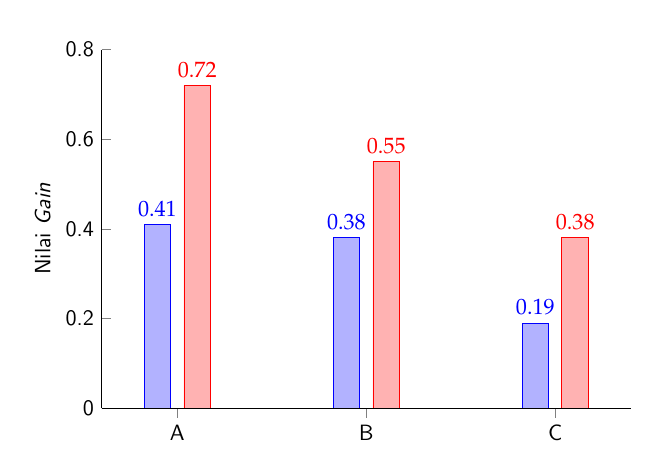
\begin{tikzpicture}[scale=0.8, transform shape]
\begin{axis}[
    every axis plot post/.style={/pgf/number format/fixed},
    ybar=6pt,
    bar width=12pt,
    x=3cm,
    ymin=0,
    axis on top,
    ylabel=Nilai \textit{Gain},
    ymax=0.8,
    xtick=data,
    enlarge x limits=0.2,
    symbolic x coords={A,B,C},
    restrict y to domain*=0:14, % Cut values off at 14
    visualization depends on=rawy\as\rawy, % Save the unclipped values
    after end axis/.code={ % Draw line indicating break
            \draw [ultra thick, white, decoration={snake, amplitude=1pt}, decorate] (rel axis cs:0,1.05) -- (rel axis cs:1,1.05);
        },
    nodes near coords={%
            \pgfmathprintnumber{\rawy}% Print unclipped values
        },
    axis lines*=left,
    clip=false
    ]
\addplot coordinates {(A,0.41) (B,0.38) (C,0.19)};
\addplot coordinates {(A,0.72) (B,0.55) (C,0.38)};
%\addplot coordinates {(A,6) (B,11) (C,7)};
\end{axis}
\end{tikzpicture}
%\includegraphics[width=0.6\textwidth]{Grafik1.pdf}
\caption{Peningkatan kemampuan pemecahan masalah untuk kelas kontrol (sebelah kiri, warna biru) dan kelas eksperimen (sebelah kanan, warna merah).
Ketrampilan yang dinilai adalah ketrampilan
(A) memahami masalah yang akan dipecahkan, (B) menyelidiki berbagai kemungkinan pemecahan masalah, dan
(C) mengevaluasi kualitas solusi pemecahan masalah.}
\label{Fig:Gain}
\end{figure}
\lipsum

\begin{figure}[htbp]
\centering
\begin{tikzpicture}
\begin{axis}
\addplot table [x=a, y=c, col sep=comma] {gambar/data.csv};
\end{axis}
\end{tikzpicture}
\caption{Ini adalah contoh grafik garis}
\end{figure}

\section{Contoh Lain}

Misalkan anda punya file:
\begin{verbatim}
\documentclass{article}

\usepackage{pgfplots}
\pgfplotsset{compat=newest}
\usetikzlibrary{calc}

\pagestyle{empty}
\usepackage{pgfplotstable}
\usepackage{mathpazo}
\usepackage[left=3.5cm, right=2cm,top=2.5cm, bottom=2cm]{geometry}
\usepackage{helvet}
\usepackage[eulergreek]{sansmath}
\pgfplotsset{
  tick label style = {font=\sansmath\sffamily},
  every axis label = {font=\sansmath\sffamily},
  legend style = {font=\sansmath\sffamily},
  label style = {font=\sansmath\sffamily}
}
\begin{document}

\input{250C}
\input{240C}

\end{document}
\end{verbatim}
Terlihat bahwa file di atas memanggil
file 250C.tex dan 240C.tex.
Isi dari file 250C.tex adalah
\begin{verbatim}
\pgfplotstableread
	{250C.csv}
	{\loadedtable}

\begin{tikzpicture}
	\begin{axis}[
	    %stack plots=y,
	    extra description/.code={\node  at  (0.8,0.85) 
                  {\bfseries (i) 250C};},
		ymin=0,
		xmax=9.5,
		minor tick num=4,
		enlarge x limits=false,
		axis on top,
		every axis plot post/.append style=
			{mark=none},
		const plot,
		xticklabels={,,},
		width=0.4\textwidth,
		height=0.3\textwidth,
%		ylabel= Load  (N),
		legend style={
			area legend,
			at={(0.5,-0.15)},
			anchor=north,
			legend columns=-1}]

%	\addplot[draw=blue,fill=blue!30!white]
	\addplot[draw=blue]
	 table[x=mm1,y=N1] from \loadedtable;
		%\closedcycle;
	\addplot table[x=mm2,y=N2] from \loadedtable;
	\addplot table[x=mm3,y=N3] 
		from \loadedtable;
	%\legend{1min load,nodes,cpus,processes}
	\end{axis}
	\pgfresetboundingbox
\useasboundingbox ($(current axis.south west)+(0,0.3ex)$)
    rectangle (current axis.north east);

\end{tikzpicture}
\end{verbatim}
Isi file 240C.tex adalah
\begin{verbatim}
\pgfplotstableread
	{240C.csv}
	{\loadedtable}

\begin{tikzpicture}
	\begin{axis}[
	    %stack plots=y,
	    extra description/.code={\node  at  (0.8,0.85) 
                  {\bfseries (ii) 240C};},
		ymin=0,
		xmax=9.5,
		minor tick num=4,
		enlarge x limits=false,
		axis on top,
		every axis plot post/.append style=
			{mark=none},
		const plot,
		xticklabels={,,},
		width=0.4\textwidth,
		height=0.3\textwidth,
%		ylabel= Load  (N),
		legend style={
			area legend,
			at={(0.5,-0.15)},
			anchor=north,
			legend columns=-1}]

%	\addplot[draw=blue,fill=blue!30!white]
	\addplot[draw=blue]
	 table[x=mm1,y=N1] from \loadedtable;
		%\closedcycle;
	\addplot table[x=mm2,y=N2] from \loadedtable;
	\addplot table[x=mm3,y=N3] 
		from \loadedtable;
	%\legend{1min load,nodes,cpus,processes}
	\end{axis}
	\pgfresetboundingbox
\useasboundingbox ($(current axis.south west)+(0,0.3ex)$)
    rectangle (current axis.north east);

\end{tikzpicture}
\end{verbatim}
Terlihat juga bahwa file 250C.tex memanggil
file 250C.csv, yang isinya kurang lebih (hanya 15 baris pertama
yang ditampilkan): 
\begin{verbatim}
No	mm1	N1	mm2	N2	mm3	N3
1	7.45E-009	30	7.45E-009	28	3.73E-009	26
2	0.02	34	0.02	36	0.02	36
3	0.03	40	0.03	36	0.03	46
4	0.05	44	0.06	52	0.05	56
5	0.07	46	0.07	58	0.06	56
6	0.09	48	0.08	58	0.08	68
7	0.1	50	0.1	70	0.1	72
8	0.12	48	0.12	72	0.12	74
9	0.13	48	0.13	72	0.14	76
10	0.15	46	0.17	76	0.15	78
11	0.17	48	0.19	78	0.17	80
12	0.18	48	0.2	80	0.18	80
13	0.2	50	0.22	82	0.2	84
14	0.22	54	0.24	86	0.22	96
15	0.23	58	0.25	90	0.24	104
\end{verbatim}
Hasilnya dapat dilihat pada Gambar~\ref{Fig:grafikTumpuk}.
\begin{figure}[htbp]
\includegraphics[width=\textwidth]{gambar/grafikTumpuk.png}
\caption{Tampilan grafik yang digabungkan secara vertikal.}
\label{Fig:grafikTumpuk}
\end{figure}

\section{Bar Graph dengan Error Bar}
\textit{Error bar} atau deviasi standar menunjukkan kualitas eksperimen.
Deviasi standar yang besar menunjukkan kualitas eksperimen yang buruk.
Namun demikian, deviasi standar tidak boleh dimanipulasi atau dimodifikasi
sehingga menjadi kecil.  Pengecilan deviasi semacam ini berbahaya karena
pada dasarnya kita tidak tahu nilai sebenarnya (yaitu nilai rata-rata) dari
eksperimen tersebut. Jika nilainya sudah diketahui, maka itu bukanlah penelitian
melainkan praktikum.

Contoh skrip \LaTeX untuk menghasilkan Gambar~\ref{Fig:bargraph-error}
adalah\footnote{Silahkan di modifikasi agar lebih menarik.}
\begin{verbatim}
      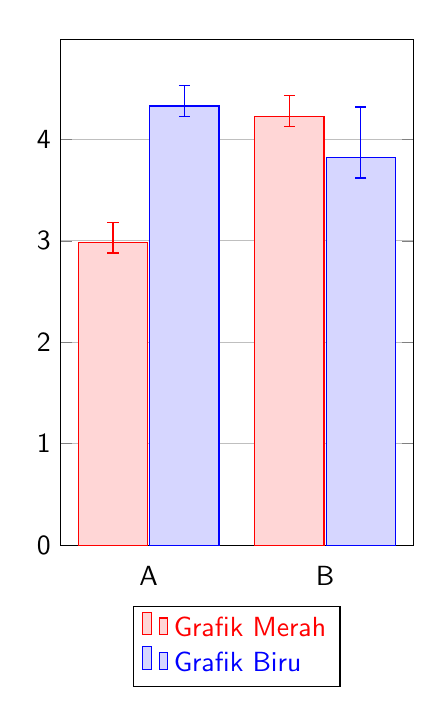
\begin{tikzpicture}
      \begin{axis}[
      width  = 0.50*\textwidth,
      height = 8cm,
      major x tick style = transparent,
      ybar=2*\pgflinewidth,
      bar width=25pt,
      ymajorgrids = true,
      symbolic x coords={A,B},
      xtick = data,
      scaled y ticks = false,
      enlarge x limits=0.50,
      ymin=0,
      legend cell align=left,
      legend style={at={(0.5,-0.12)},anchor=north},
  ]
      \addplot[red,style={fill=red!80!white!20},
error bars/.cd, y dir=both, y explicit]
          coordinates {
          (A, 2.98) += (0,0.2) -= (0,0.1)
          (B,4.23) += (0,0.2) -= (0,0.1)};

      \addplot[style={blue,fill=blue!80!white!20},
error bars/.cd, y dir=both, y explicit,error bar style=blue]
           coordinates {
           (A,4.33) += (0,0.2) -= (0,0.1)
           (B,3.82) += (0,0.5) -= (0,0.2)};

      \legend{\textcolor{red}{Grafik Merah}, \textcolor{blue}{Grafik Biru}}
  \end{axis}
  \end{tikzpicture}
\end{verbatim}
\begin{figure}[htbp]
        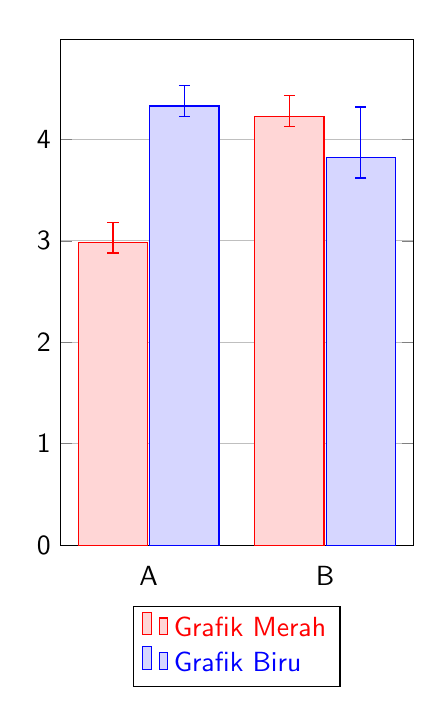
\begin{tikzpicture}
      \begin{axis}[
      width  = 0.50*\textwidth,
      height = 8cm,
      major x tick style = transparent,
      ybar=2*\pgflinewidth,
      bar width=25pt,
      ymajorgrids = true,
      symbolic x coords={A,B},
      xtick = data,
      scaled y ticks = false,
      enlarge x limits=0.50,
      ymin=0,
      legend cell align=left,
      legend style={at={(0.5,-0.12)},anchor=north},
  ]
      \addplot[red,style={fill=red!80!white!20},error bars/.cd, y dir=both, y explicit]
          coordinates {
          (A, 2.98) += (0,0.2) -= (0,0.1)
          (B,4.23) += (0,0.2) -= (0,0.1)};

      \addplot[style={blue,fill=blue!80!white!20},error bars/.cd, y dir=both, y explicit,error bar style=blue]
           coordinates {
           (A,4.33) += (0,0.2) -= (0,0.1)
           (B,3.82) += (0,0.5) -= (0,0.2)};

      \legend{\textcolor{red}{Grafik Merah}, \textcolor{blue}{Grafik Biru}}
  \end{axis}
  \end{tikzpicture}

  \caption{\textit{Bar-graph} berikut \textit{error bar}.}
  \label{Fig:bargraph-error}
\end{figure}
